\documentclass{article}

%%%%%%%%%%%%%%%%%%%%%%%%%%%%%%%%%%%%%%%%%%%%%%%%%%%%%
%                                                   %
%              Template by Tuur Vanhoutte           %
% https://github.com/zjeffer/howest-thesis-template %
%                                                   % 
%%%%%%%%%%%%%%%%%%%%%%%%%%%%%%%%%%%%%%%%%%%%%%%%%%%%%

%%%%% Package importing %%%%%
\usepackage[english]{babel}
\usepackage[margin=2.5cm]{geometry}
\usepackage{graphicx}
\usepackage{float}
\usepackage{caption}
\usepackage{hyperref}
\usepackage{amsmath}
\usepackage{wrapfig}
\usepackage[parfill]{parskip}
\usepackage{eso-pic}
\usepackage{titlesec}
\usepackage{titletoc}
\usepackage{tcolorbox}
\usepackage{enumitem}
\usepackage{changepage}

\usepackage{bookmark}
\usepackage{csquotes}
\usepackage[style=ieee]{biblatex}
\addbibresource{sources.bib}


%%%%% Change fonts here %%%%%
\usepackage[T1]{fontenc}
\usepackage{helvet}
\renewcommand{\familydefault}{\sfdefault}

\graphicspath{{img/}}

%%%%% \theorem environment %%%%%
\usepackage{amssymb}
\newtheorem{theorem}{Definition}[section]
\newenvironment{thmenum}
 {\begin{enumerate}[label=\upshape\bfseries(\roman*)]}
 {\end{enumerate}}


%%%%% Styled code block %%%%%
\usepackage{minted}
\setminted{frame=single,framesep=3pt,linenos}
\usepackage{upquote}
\usepackage{color}

%%%%% TOC styling %%%%%
\makeatletter
\renewcommand\tableofcontents{%
  \null\hfill\textbf{\Huge\contentsname}\hfill\null\par
  \vline\noexpand\rule{\textwidth}{1pt}%
  \@mkboth{\MakeUppercase\contentsname}{\MakeUppercase\contentsname}%
  \@starttoc{toc}%
}
\makeatother

\begin{document}

%%%%% title page %%%%%
\begin{titlepage}
    \newgeometry{margin=0cm}
    \begin{center}
        %%%%% Change the cover image here %%%%%
        \includegraphics[width=18.5cm,height=18.5cm]{example-image}
    \end{center}
    \begin{adjustwidth}{1.5cm}{1.5cm}

    \vspace{0.5em}

    \MakeUppercase{\Huge\textbf{How to create a chess engine using Deep Reinforcement Learning}}

    \MakeUppercase{\Large\textit{A critical look at DeepMind's AlphaZero}}

    \vspace{1em}

    \MakeUppercase{Internal promotor: Wouter Gevaert}

    \MakeUppercase{External promotor: <name here>}

    \vspace{1em}

    \MakeUppercase{\small{Research conducted by}}

    \MakeUppercase{\Large\textbf{{Tuur Vanhoutte}}}

    \MakeUppercase{\small{for obtaining a bachelor's degree in}}

    \MakeUppercase{\Large{\textbf{{Multimedia \& Creative Technologies}}}}

    \MakeUppercase{Howest | 2021-2022}
    \end{adjustwidth}
\end{titlepage}

\newgeometry{margin=2.5cm}

\newpage
\thispagestyle{empty}
\mbox{}
\newpage

%%%%% Set pagenumbering off %%%%%
\pagenumbering{arabic}
\thispagestyle{empty}
%%%%% Preface %%%%%
\section*{Preface}
\addcontentsline{toc}{section}{Preface}

This bachelor thesis is the conclusion to the bachelor program Multimedia \& Creative Technologies at Howest college
West Flanders in Kortrijk, Belgium. The program teaches students a wide range of skills in the field of 
computer science, with a focus on creativity and Internet of Things. From the second year on, students can choose 
between four different modules:

\begin{enumerate}
    \item \textbf{AI Engineer}
    \item \textbf{Smart XR Developer}
    \item \textbf{Next Web Developer}
    \item \textbf{IoT Infrastructure Engineer}
\end{enumerate}

This bachelor thesis was made under the \textbf{AI Engineer} module.
The subject of the thesis is a critical look at the result of my research project 
in the previous semester. The goal of the project was to create a chess engine in Python with
deep reinforcement learning based on DeepMind's AlphaZero algorithm. 

I will explain the research I needed to create it, the technical details on how to program the
chess engine and I will reflect on the results of the project. To do this, I will contact 
multiple people and communities familiar with the field of reinforcement learning to get a better understanding of the
impact of this research on society. Based on this, I will give advice to people and companies who 
wish to implement similar algorithms.

I would like to show gratitude to Wouter Gevaert for his enthusiastic support in the creation of my research project 
and this thesis. I also want to thank the other teachers at Howest Kortrijk, who shared their knowledge
and expertise in programming and AI in very interesting classes.

% TODO: thank external promotor

Furthermore, I would like to thank my parents for giving me the chance to have a good education, and 
the motivation to get the best I can out of my studies.

\vspace{3em}

\begin{center}
    \textbf{Tuur Vanhoutte}, 1$^{\text{st}}$ June 2022 % TODO: verander datum naar datum finale versie
\end{center}

\newpage
\thispagestyle{empty}
\mbox{}
\newpage

%%%%% Abstract %%%%%
\section*{Abstract}
\addcontentsline{toc}{section}{Abstract}


% Samenvatting of abstract (mag in het Engels): MAX 1 halve A4-pagina: 
% Je beantwoordt in de samenvatting kort en bondig een viertal vragen: 
% X Wat is de onderzoeksvraag?
% X Wat was jouw onderzoek? 
% - Welke elementen spelen een grote rol (zowel positief als negatief) bij de evaluatie van het onderzoek? 
% - Welke elementen zijn belangrijk bij jouw advies?
% - Het besluit wordt kort samengevat

This bachelor thesis answers the question: ``How to create a chess engine using deep reinforcement learning?''.
It explains the difference between normal chess engines and chess engines that use deep reinforcement learning, and
specifically tries to recreate the results of AlphaZero, the chess engine by DeepMind, in Python on consumer hardware. 

The technical research shows what is needed to create my implementation using Python and TensorFlow. 
It shows how to program the chess engine, how to build the neural network, and how to train and evaluate the network.
During the creation of this chess engine, it was crucial to create a huge amount of data through self-play.

% TODO: abstract volledig herschrijven vanaf hier

The thesis contains a reflection on the results of my research project, which proposes a solution to the problem of
creating a high amount of games through self-play. It also reflects on the impact of this research on society, and the
viability of this type of artificial intelligence in the future. It follows with advice to people and companies who wish to implement similar algorithms. 

% TODO: CONCLUSION


\newpage
\thispagestyle{empty}
\mbox{}
\newpage

%%%%% Table of contents %%%%%
\addcontentsline{toc}{section}{Contents}
\tableofcontents
\newpage

%%%%% List of figures %%%%%
\section*{List of figures}
\addcontentsline{toc}{section}{List of figures}
\renewcommand{\listfigurename}{}
\listoffigures
\newpage

% TODO: Remove if no tables
\section*{List of tables}
\addcontentsline{toc}{section}{List of tables}
\renewcommand{\listtablename}{}
\listoftables

%%%%% List of abbreviations %%%%%
\section*{List of abbreviations}
\addcontentsline{toc}{section}{List of abbreviations}



%%%%% Glossary %%%%%
\newpage
\section*{Glossary}
\addcontentsline{toc}{section}{Glossary}

%%%%% Introduction %%%%%
\newpage
\setcounter{section}{0}
\section{Introduction}

% Doel: In de inleiding beschrijf je ook hoe jouw bachelorproef in elkaar steekt. Een krachtige heldere inleiding 
% zorgt ervoor dat je de lezer voor je wint en hij/zij sneller de rest van jouw document zal gaan lezen. 
% In de inleiding introduceer je de onderzoeksvraag. Je vermeldt de achtergrond of bestaande situatie. Je licht toe 
% waarom de onderzoeksvraag voor jou/jouw stagebedrijf relevant is. Ook eventuele deelvragen worden 
% nauwgezet omschreven. 
% De inleiding omschrijft ook de gebruikte onderzoeksmethode. Je legt uit waar, wanneer, met wie en hoe je het 
% onderzoek gaat doen. 
% Je kunt alvast gebruikmaken van één of meerdere standaardzinnen: 
% - De data voor dit onderzoek zijn verzameld door... 
% - Vijf stukken worden onderzocht, die allemaal... 
% - De onderzoeksgegevens in deze bachelorproef zijn afkomstig uit vier belangrijke bronnen, namelijk... 
% - Door kwalitatieve methoden te gebruiken probeer ik... uiteen te zetten/uit te lichten. 
% - De studie is uitgevoerd in de vorm van een enquête, waarbij data zijn verzameld via... 
% - De methode die in deze studie gebruikt is, is een gemengde aanpak gebaseerd op...

Chess is not only one of the most popular board games in the world, it is also a breeding ground for
complex algorithms and more recently, machine learning. Chess is theoretically a deterministic game: 
no information is hidden from either player and every position has a calculable set of possible moves.
Because the branching factor of chess is about 35-38 moves \cite{BranchingFactorChessprogramming}, 
calculating if a position is winning or losing requires an enormous amount of calculations.

Throughout the entire history of computer science, researchers have continuously tried to find better
ways to calculate if a position is winning or losing. The most famous example is the StockFish 
engine \cite{StockfishChess2022}, which uses the minimax algorithm with alpha-beta pruning to calculate the best move.

Recently, researchers at Google DeepMind have developed a new algorithm called AlphaZero \cite{AlphaZero2022}.
This thesis explores the concept of AlphaZero, how to create a chess engine based on it, and the impact of 
the algorithm on both the world of chess and the rest of society.

Research has been conducted by investigating what is needed to recreate the results of AlphaZero, 
by programming a simple implementation using Python and TensorFlow Keras. This was done as part of a research project
between November 2021 and January 2022. The code was written with lots of trial and error, as DeepMind released 
very little information about the detailed workings of the algorithm. It also only released a simple version of 
the algorithm in pseudocode, so it isn't possible to directly compare AlphaZero with other chess engines.

As I have been playing chess for most of my life, I was naturally very interested in the workings of AlphaZero
and why it worked so well against the StockFish engine. Because AlphaZero was trained on supercomputers, 
I wanted to investigate where its flaws lie when implementing it in Python on consumer hardware.


%%%%% Add Howest background %%%%%
\AddToShipoutPicture{
    \ifnum\value{page}>0
    \AtPageLowerLeft{
    \raisebox{3\baselineskip}{\makebox[0.25\paperwidth]{
        \begin{minipage}{21cm}\centering
            
\includegraphics{img/background.png}
        \end{minipage}}}
    }
  \fi
}

%%%%% Research %%%%%
\newpage
\section{Research}

%%%%%%%%%%%%% 
% 
% Answer the theoretical questions:
%
% [X] Hoe kan ik het Monte Carlo Tree Search algoritme gebruiken om de beste zetten te selecteren?
% [X] Welke voordelen biedt deep reinforcement learning bij schaken?
% [X] Hoe ziet de architectuur van het neurale netwerk er uit?
% [X] Hoe werd deep reinforcement learning reeds gebruikt bij andere spellen?
% [X] Hoe werken huidige schaakcomputers die geen neurale netwerken gebruiken?
%
%%%%%%%%%%%%%

\subsection{What is a chess engine?}

According to Wikipedia \cite{ChessEngine2022}, a chess engine is a computer program that analyzes 
chess or chess variant positions, and generates a move or list of moves that it regards as strongest.
Given any chess position, the engine will estimate the winner of that position based on the strength 
of the possible future moves up to a certain depth. The strength of a chess engine is determined by
the amount of moves, both in depth and breadth, that the engine can calculate. 


\subsection{How do traditional chess engines work?}

Contemporary chess engines, like StockFish \cite{StockfishChess2022}, use a variant of the minimax algorithm that employs alpha-beta pruning.

\subsubsection{The minimax algorithm}

The minimax algorithm \cite{Minimax2022} is a general algorithm usable in many applications, ranging from artificial intelligence to 
decision theory and game theory. The algorithm tries to minimize the maximum amount of loss. In chess, this means 
that the engine tries to minimize the possibility for the worst-case scenario: the opponent
checkmating the player. For games where the player needs to maximize a score, the algorithm is called maximin: 
maximizing the minimum gain. 

Minimax recursively creates a search tree \cite{eppesHowComputerizedChess2019}, with chess positions as nodes and chess moves as edges between the nodes. 
Each node has a value that represents the strength of the position for the current player. 
At the start of the algorithm, the tree only consists of a root node that represents the current position. 
It then explores the tree in a depth-first manner by continuously choosing random legal moves, creating nodes and edges in the process.

This means that it will traverse the tree vertically until a certain depth is reached:

\begin{figure}[H]
    \centering
    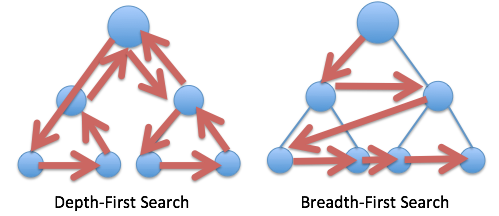
\includegraphics[width=0.5\textwidth]{img/depth-vs-breadth.png}
    \caption{Depth-First search vs Breadth-First search \cite{eppesHowComputerizedChess2019}}
\end{figure}

When that happens, that leaf node's position is evaluated and its value is returned
upwards to the parent node. The parent node looks at all of its children's values, 
and receives the maximum value when playing white, and the minimum value
when playing black. 

This repeats until the root node receives a value: the strength of the current position.

\subsubsection{The evaluation function}

The value estimation of leaf nodes is done by an evaluation function \cite{EvaluationFunction2022} written specifically
for the game. This function can differ from engine to engine, and is usually written with 
help from chess grandmasters. 



\subsubsection{Pseudocode}

The algorithm is recursive; it calls itself with different arguments, depending
on which player's turn it is. In chess, white wants to maximize the score, and 
black wants to minimize it. \cite{Minimax2022}

\begin{minted}{c}
function  minimax(node, depth, maximizingPlayer) is
    if depth = 0 or node is a terminal node then
        return the heuristic value of node
    if maximizingPlayer then
        value := - inf
        for each child of node do
            value := max(value, minimax(child, depth - 1, FALSE))
        return value
    else (* minimizing player *)
        value := + inf
        for each child of node do
            value := min(value, minimax(child, depth - 1, TRUE))
        return value
\end{minted}

Calling the function:

\begin{minted}{c}
// origin = node to start
// depth = depth limit
// maximizingPlayer = TRUE if white, FALSE if black
minimax(origin, depth, TRUE)
\end{minted}

\subsubsection{Alpha-beta pruning}

Because the necessary amount of nodes to get a good estimation of the strength of a position
is so high, the algorithm needs to be optimized. 
Alpha-beta pruning \cite{AlphaBetaPruning2022} aims to reduce the amount of nodes that need to be explored by minimax.
It does this by cutting off branches in the search tree that lead to worse outcomes.

Say you're playing the white pieces. You want to minimize your maximum loss, which means 
you want to make sure that black's score is as low as possible. 
Minimax always assumes that the opponent will play the best possible move. If one of white's possible moves
leads to a position where black gets a big advantage, it will eliminate that branch of the search tree.
As a result, the amount of nodes to explore is greatly reduced, while retaining a good estimation 
of the strength of the position.

\subsection{Monte Carlo Tree Search}

The biggest problem with minimax algorithms that use a depth limit is the dependency on the evaluation function.
If the evaluation function makes incorrect or suboptimal estimations, the algorithm will suggest bad moves. 
Developers of contemporary chess engines like StockFish continuously try to improve this function. 
Since 2020, StockFish has been using a sparse and shallow neural network as its evaluation function. 
This neural network is still trained using supervised learning, not (deep) reinforcement learning.

Using alpha-beta pruning can also bring about some problems. Say the player can sacrifice a piece
to get a huge advantage later in the game. The algorithm might cut off the branch and never explore that winning line, 
because it considers the sacrifice a losing position \cite{MinimaxMonteCarlo}. 

Monte Carlo Tree Search (MCTS) \cite{MonteCarloTree2022} is a search algorithm that can be used to mitigate these problems.
MCTS approximates the value of a position by creating a search tree using random exploration of the most promising moves.

\subsubsection{The algorithm}

To create this search tree for a certain position, MCTS will run the following algorithm hundreds of times. 
Each of these runs is called an MCTS \textbf{simulation}. One simulation consists of four steps:

\begin{enumerate}
    \item \textbf{Selection}:
    \begin{itemize}
        \item Starting from the root node, select a child node based on a formula of your choice.
        \item Most implementations of MCTS use some variant of Upper Confidence Bound (UCB) \cite{MLMonteCarlo2019}
        \item Keep selecting nodes until a node has been reached that has not been visited (=expanded) before. We call this a leaf node.
        \item If the root node is a leaf node, we immediately proceed to the next step.
    \end{itemize}
    \item \textbf{Expansion}:
    \begin{itemize}
        \item If the selected leaf node is a terminal node (the game ends), proceed to the backpropagation step.
        \item If it doesn't, create a child node for every possible action that can be taken from the selected node.
    \end{itemize}
    \item \textbf{Simulation}:
    \begin{itemize}
        \item Choose a random child node that was expanded in the previous step.
        \item By only choosing random moves, simulate the rest of the game from that child node's position.
    \end{itemize}
    \item \textbf{Backpropagation}:
    \begin{itemize}
        \item Return the simulation's result up the tree.
        \item Every node tracks the number of times it has been visited, and the number of times it has lead to a win.
    \end{itemize}
\end{enumerate}


\begin{figure}[H]
    \centering
    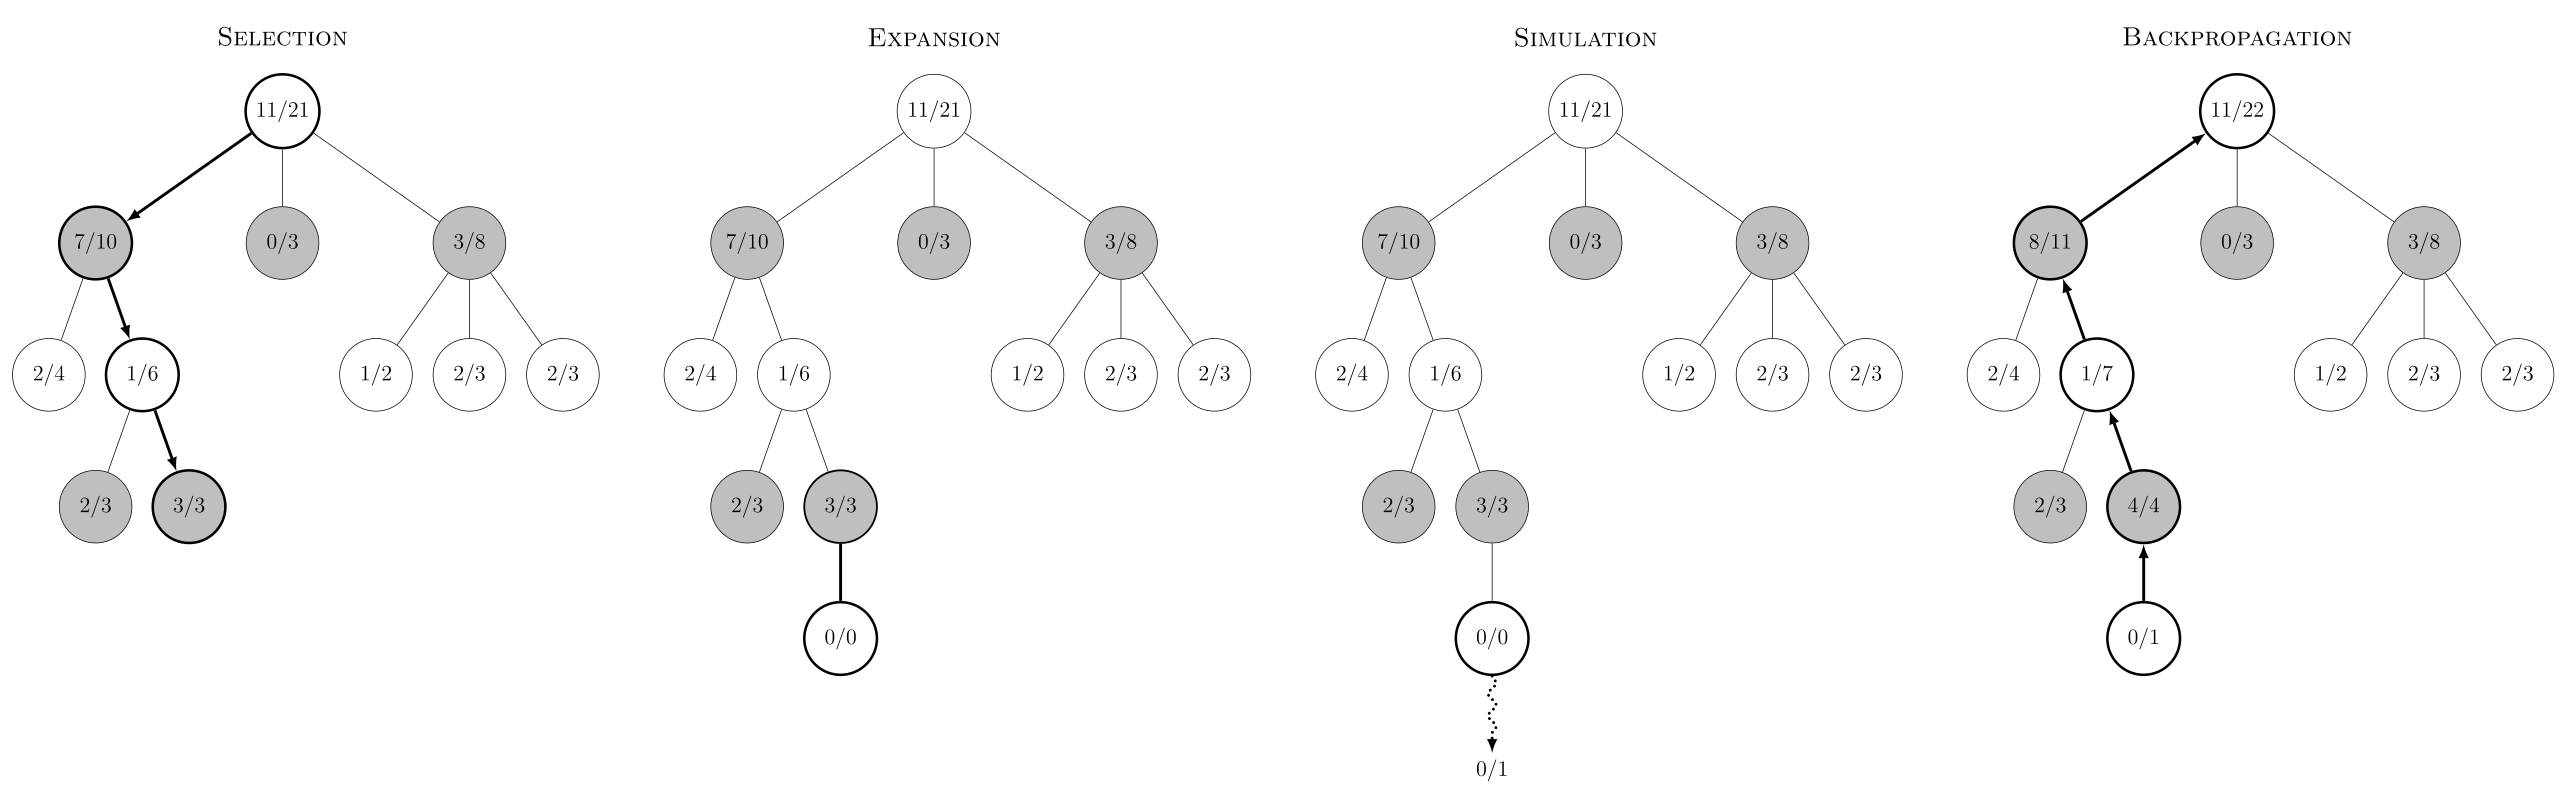
\includegraphics[width=0.98\textwidth]{img/MCTS-steps.png}
    \caption{The 4 steps of the MCTS algorithm \cite{MonteCarloTree2022}}
\end{figure}

For chess, this algorithm is very inefficient, because of its necessity to simulate 
an entire game of chess in the third step of every simulation. 
Just to calculate the value of one position would need hundreds of these simulations to get a good estimation.
This is why the selection formula needs to be chosen carefully; it's important to select nodes in a way that
balances exploration and exploitation.

\subsection{Go}

Go is a Chinese two-player strategy board game that uses white and black stones as playing pieces \cite{GoGame2022}.
It is played on a rectangular grid of (usually) 19 by 19 lines. The rules are relatively simple, but due to 
its extremely complex possibilities, Go has been a very popular playground for AI research similarly to chess.
Go's much larger branching factor compared to chess makes it very difficult to evaluate a position using 
traditional methods like minimax with alpha-beta pruning.

\begin{figure}[H]
    \centering
    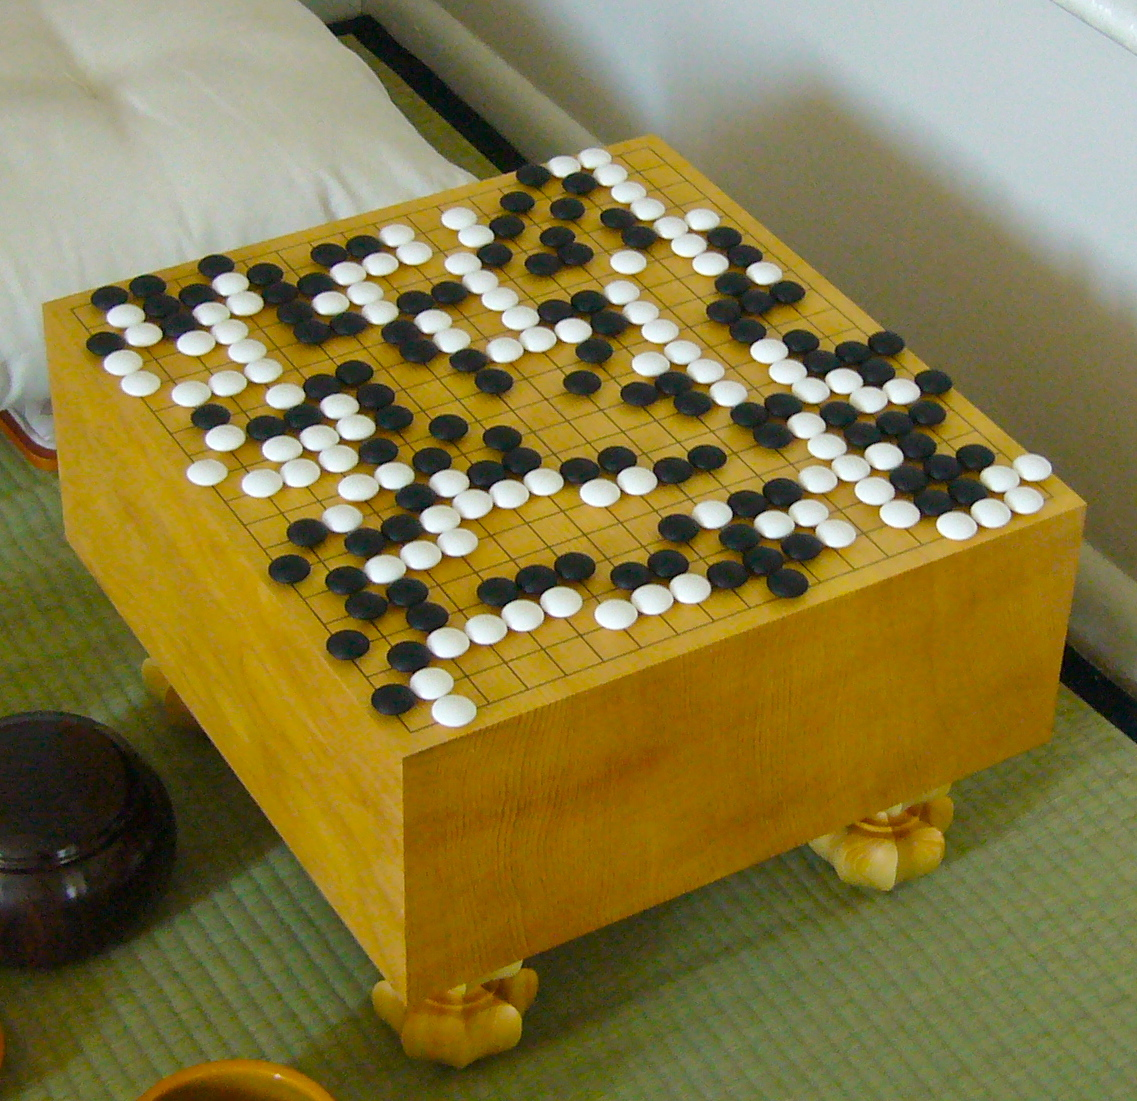
\includegraphics[width=0.5\textwidth]{img/go.jpg}
    \caption{Go board \cite{GoGame2022}}
\end{figure}

\subsubsection{AlphaGo}

In 2014, DeepMind Technologies \cite{DeepMind2022}, a subsidiary of Google, 
started developing a new algorithm called AlphaGo to play Go \cite{AlphaGo2022a}. 
Previously, the strongest Go engines were still only good enough to win against amateur Go players \cite{AlphaGo}.
The algorithm used a combination of the MCTS algorithm and a deep neural network to evaluate positions. 

AlphaGo was built \cite{AlphaGo, MasteringGameGo}  by first training a neural network with supervised learning by using data from human games.
The weights of that network were then copied to a new reinforcement learning network. That network was used to 
create a training set through self-play. By playing against itself and recording the board state, the 
moves the network considered, and the eventual winner of the game, a training set was created.
That training set was then used to train the reinforcement learning network. A separate network (the value network) 
was used to estimate the value of a position. 

\subsubsection{AlphaGo Zero}

Because AlphaGo still used some amateur games to learn from, the next step was creating a version of AlphaGo
that learns completely from scratch. That's why DeepMind developed AlphaGo Zero \cite{AlphaGoZero2022}.
AlphaGo Zero uses a different kind of network than AlphaGo. Instead of using two separate networks, 
it will combine the two outputs into a policy head and a value head. It's also using different layers:
residual layers instead of convolutional layers \cite{MasteringGameZero}. 

\subsection{AlphaZero}

AlphaZero is a generalized version of AlphaGo Zero, created to master the games of chess, shogi (``Japanese chess''), and Go \cite{AlphaZero2022, silverMasteringChessShogi2017a}. 
For chess, AlphaZero was evaluated against StockFish version 8 by playing 1000 games with 3 hours per player, plus 
15 seconds per move. It won 155 times, lost 6 times and the remaining games were drawn. 
AlphaZero uses a single neural network with two outputs, just like AlphaGo Zero. 


\subsubsection{Neural network input}

The input to the network represents the state of the game. 
It has the following shape: $N \cdot N \cdot (M \cdot T + L)$:

\begin{itemize}
    \item $N$ is the board size
    \begin{itemize}
        \item $N = 8$ in chess.
    \end{itemize}
    \item $M$ is the number of different pieces on the board, 
    \begin{itemize}
        \item Two players with six types of pieces each
        \item Every piece is represented by its own 8x8 board of boolean values
        \item For every square: $1$ if the piece is on that square, $0$ if it isn't
        \item $M = 12$ in chess
    \end{itemize}
    \item $T$ is the amount of previous moves that are used as input, including the current move. 
    \begin{itemize}
        \item AlphaZero used $T = 8$ for both chess, shogi, and Go.
        \item This gives the network a certain history to learn from
    \end{itemize}
    \item $L$ represents a set of rules specific to the game
    \begin{itemize}
        \item $L = 7$ in chess
        \item $1$ plane to indicate whose turn it is
        \item $1$ for the total amount of moves played so far
        \item $4$ for castling legality (white and black can both castle kingside or queenside under certain conditions)
        \item $1$ to represent a repetition count (in chess, 3 repetitions results in a draw)
    \end{itemize}
    \item $\Rightarrow 8 \cdot 8 \cdot (12 \cdot 8 + 7)$. 
\end{itemize}

This means that the input to the neural network is 119 8x8 boards of boolean values.

\subsubsection{Neural network layers}

DeepMind tested multiple neural network architectures for AlphaGo Zero \cite{NeuralNetworksChessprogramming}. 
The following parts were used in these networks:

\begin{itemize}
    \item Convolutional block
    \begin{itemize}
        \item A convolution layer
        \item Batch normalization layer
        \item ReLu activation function
    \end{itemize}
    \item Residual block
    \begin{itemize}
        \item This consists of two convolutional blocks, and a skip-connection
        \item The skip-connection will combine the input of the block to the output of the first two convolutional blocks
    \end{itemize}
\end{itemize}

These networks were tested by DeepMind during development of AlphaGo Zero \cite{MasteringGameZero}:

\begin{enumerate}
    \item \textbf{`dual-res':} a single tower of 20 residual blocks with combined policy and value heads. This is the architecture used in AlphaGo Zero.
    \item \textbf{`sep-res':} two towers of 20 residual blocks each: one with the policy head and one with the value head.
    \item \textbf{`dual-conv':} a single tower of 12 convolutional blocks with combined policy and value heads.
    \item \textbf{`sep-conv':} two towers of 12 convolutional blocks each: one with the policy head and one with the value head. This is the network used in AlphaGo.
\end{enumerate}

AlphaZero uses the same network architecture as AlphaGo Zero: dual-res.

\subsubsection{Neural network output}

The neural network has two outputs:

\begin{itemize}
    \item A policy head, which represents a probability distribution over the possible actions.
    \item A value head, which represents the value of the current position.
\end{itemize}

While the value head simply outputs a single float value between -1 and 1, the policy head is quite a bit more complicated.
It outputs a vector of probabilities, one for each possible action in the chosen game. 
For chess, 73 different types of actions are possible:

\begin{itemize}
    \item 56 possible types of ``queen-like'' moves: 8 directions to move the piece a distance between 1 and 7 squares.
    \item 8 possible knight moves
    \item 9 special ``underpromotion'' moves:
    \begin{itemize}
        \item If a pawn is promoted to a queen, it is counted as a queen-like move (see above)
        \item If a pawn is promoted to a rook, bishop, or knight, it is seen as an underpromotion (3 pieces)
        \item 3 ways to promote: pushing the pawn up to the final rank, or diagonally taking a piece and landing on the final rank
        \item $\Rightarrow 3 \cdot 3 = 9$
    \end{itemize}
\end{itemize}

These 73 actions are each represented by a plane of 8x8 float values. Say the first plane is a queen-like move
to move a piece one square northwest, the second plane could be the same type of move, but a distance of two squares, and so on.
The squares on these planes represent the square from which to pick up a piece. 

% TODO: example

The result is a $73 \cdot 8 \cdot 8$ vector of probabilities, so $4672$ float values.  

\subsection{Training the network}

To train this type of network, it's necessary to create a large dataset. 
This is done by letting the engine play against itself for a high amount of matches. 
For every action taken by the agent, data is collected and stored in the training set.
For complex games like chess, shogi and Go, this training set needs to be huge
because of the extremely large amount of possible situations.

\subsubsection{Tensor Processing Units (TPU)}

Because of the requirement to play a high amount of matches against itself, it was necessary to calculate
MCTS simulations in parallel on as fast as possible hardware. 
To help with these calculations, DeepMind used Google's newly created Tensor Processing Units (TPU) \cite{TensorProcessingUnit2022}.
A TPU is an application-specific integrated circuit (ASIC \cite{ApplicationspecificIntegratedCircuit2022}) that is specifically built for machine learning with
neural networks. Since 2018, these TPUs have been made publicly available to rent through Google's Cloud Platform. Smaller TPUs 
can be purchased from Google. 

\subsection{Leela Chess Zero}

Leela Chess Zero (lc0) is a free, open-source project that attempts to replicate the results of AlphaZero \cite{LeelaChessZero2022}. 
Lc0 was adapted from Leela Zero \cite{LeelaZero2021}, a Go computer that attempted to replicate the results AlphaGo Zero \cite{AlphaGoZero2022}. 

It is written in C++ \cite{Lc02022}, and it has managed to play at a level that is comparable to the current best version of StockFish.
Because lc0 is a community driven project, volunteers can help create training games through self-play using their own computers.
This made it possible to feed millions of chess games into the network. 

%%%%% Technical research %%%%%
\newpage
\section{Technical research}

% Volgende zaken worden verwacht:
% Beschrijving van de ontwikkelde software
% Opbouw applicatie: structuur/opbouw van het resultaat
% Achterliggende technologieën
% Overwonnen moeilijkheden/problemen
% …

\subsection{Introduction}

Creating the chess engine required programming the following parts:

\begin{itemize}
    \item The MCTS algorithm
    \item A tree data structure with nodes and edges
    \item The neural network
    \item The training pipeline
    \item The evaluation pipeline
    \item A way to store every move to a dataset
    \item A class to make the engine play against itself
    \item A GUI to play against the engine
    \item Docker containers for easily scaling and distributing the program
\end{itemize}

All code was written in Python. The neural network was made using the TensorFlow Keras library.
Chess rules and helper functions were implemented using the open-source library python-chess \cite{PythonchessChessLibrarya}.

\subsection{Class structure}

\begin{figure}[H]
    \centering
    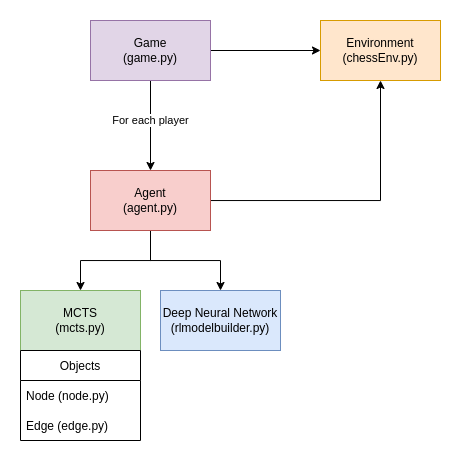
\includegraphics[width=0.6\textwidth]{img/class-structure.png}
    \caption{Basic class structure for the code responsible for playing a game}
\end{figure}

\subsubsection{Making one move}

\begin{figure}[H]
    \centering
    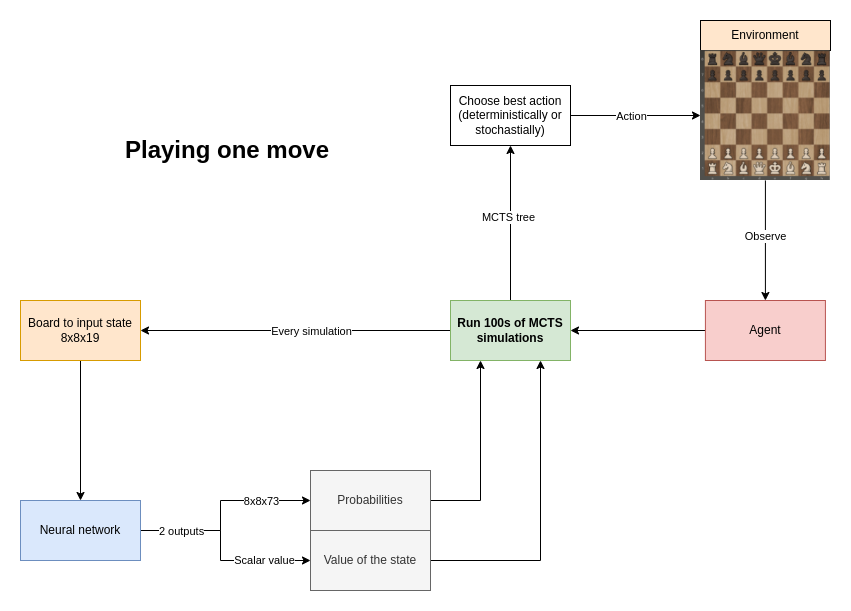
\includegraphics[width=0.95\textwidth]{img/ChessRL-schematic.png}
    \caption{Pipeline to make one move}
\end{figure}

To make a move, an Agent (white or black) observes the environment: the chessboard.
The agent calls upon the MCTS class to create a tree with as root the current state of the chessboard.
The MCTS class will run the MCTS algorithm hundreds of times. This amount is configurable in the config file. 
Higher amounts result in a more accurate estimation of the position's value, but also in longer 
computation times.

Every MCTS simulation, the neural network will be called to evaluate a position. The two outputs, 
the policy and the value, will be used to update the tree. 

\begin{figure}[H]
    \centering
    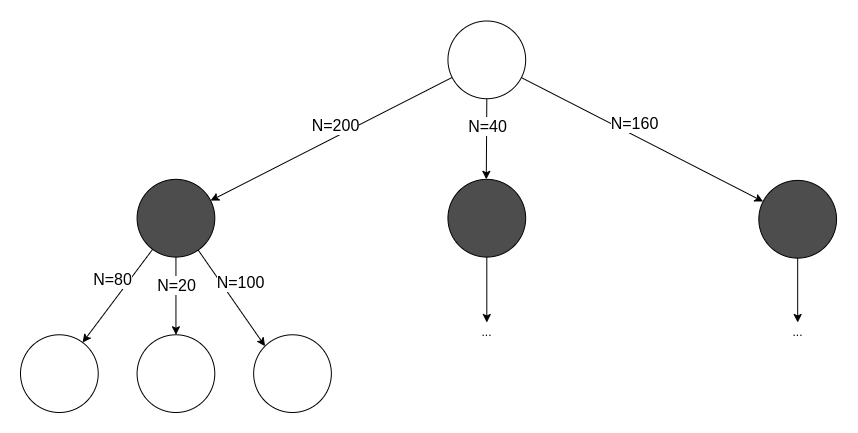
\includegraphics[width=0.65\textwidth]{img/MCTS-choose-move.png}
    \caption{Example tree after 400 simulations. N = amount of times the selection step selects that edge}
\end{figure}

After the simulations are done, the agent will pick the best move from the tree. 
It can do this in two ways:

\begin{itemize}
    \item Deterministically: choosing the most visited move 
    \item Stochastically: creating a uniform distribution of the visit counts and picking a move from that distribution
\end{itemize}

Stochastic selection is better when creating a training set, as it will result in a more diverse dataset.
Deterministic selection is better when evaluating with a previous network, or playing against the network competitively. 
In that case, picking the most visited move is the best choice.


\subsection{The neural network}

Initially, a prototype of the neural network was created with randomly initialized weights.
The Python class to create the model was immediately made with customizability in mind: 
the input and output shapes can be given as arguments, and the sizes of the convolution filters 
can be changed using a configuration file.

The neural network architecture is the same as AlphaZero's (see the Research section). 

\subsection{A tree structure with nodes and edges}

As mentioned before, the MCTS algorithm creates a tree structure to represent 
the possible future states after the current position.

Node and Edge classes were written. The Node class represents a position in the game, and
holds the following data:

\begin{itemize}
    \item The position: a string representation of the board using the Forsyth-Edwards Notation (FEN) \cite{ForsythEdwardsNotation2022}
    \item The current player to move (boolean)
    \item A list of edges connected to this node
    \item The visit count of this node, initialized to 0
    \item The value for this node, initialized to 0
\end{itemize}

The Edge class represents a move. It holds the following data:

\begin{itemize}
    \item The input node (the position from which the move was made)
    \item The output node (the resulting position after taking the move)
    \item The move itself: an object of the Move class from the python-chess library, which holds:
    \begin{itemize}
        \item The source square and the target square of the move
        \item If the move was a promotion: the piece it was promoted to
    \end{itemize}
    \item The prior probability of this move
    \item The visit count of this edge, initialized to 0
    \item The value for this action, initialized to 0
\end{itemize}

The tree can also be plotted using the Graphviz library \cite{Graphviz}. A recursive function was written to 
create the tree and output it to an SVG file. 

\subsection{The MCTS algorithm}


\begin{figure}[H]
    \centering
    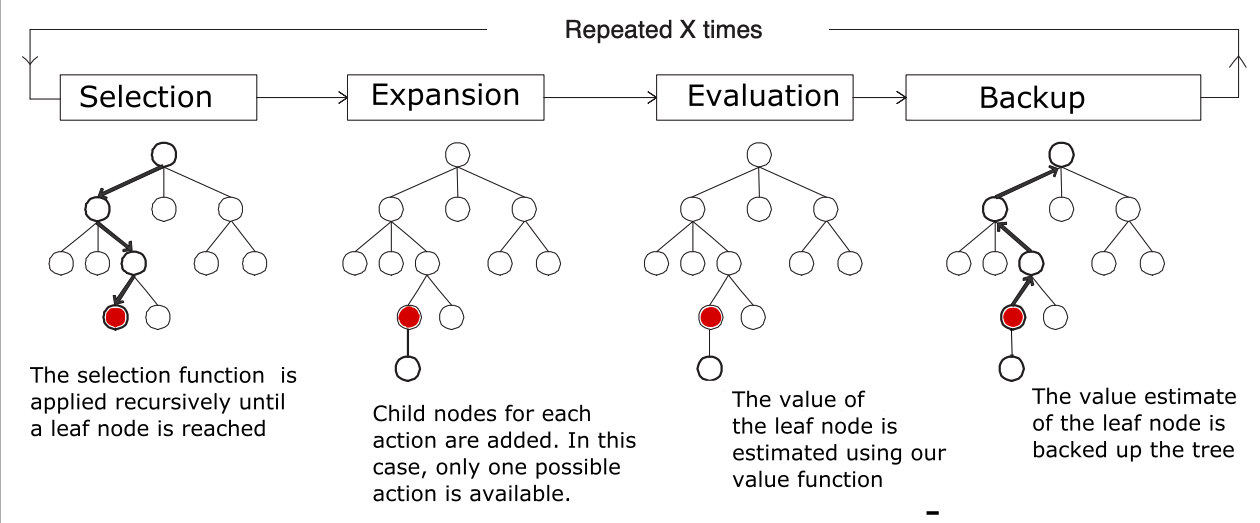
\includegraphics[width=0.9\textwidth]{img/mcts-alphazero.png}
    \caption{The four steps in AlphaZero's MCTS algorithm \cite{bodensteinAlphaZero2019}}
\end{figure}

A class was written to hold an MCTS tree. It holds the agent who created the tree and the
current position as the root node. 

\subsubsection{The selection step}

For the selection step, the following UCB formula \cite{silverMasteringChessShogi2017a} was used to determine which edge to select:

\begin{center}
    \begin{equation}
        UCB = \Big(\log({\frac{(1 + N_{\text{parent}} + C_{\text{base}})}{C_{\text{base}}}}) + C_{\text{init}}\Big) \cdot P \cdot \frac{\sqrt{N_\text{parent}}}{(1 + N)}
    \end{equation}
\end{center}

\begin{itemize} 
    \item $C_{\text{base}}$ and $C_{\text{init}}$ are constants that can be changed in the config file. The same values as AlphaZero were used.
    \item $N_{\text{parent}}$ is the visit count of the input node
    \item $N$ is the visit count of the edge
    \item $P$ is the prior probability of the edge
\end{itemize}

The selection step combines this UCB formula with the edges action-value and visit count:

\begin{center}
    \begin{equation}
        Q = \frac{W}{N+1}
    \end{equation}
\end{center}

\begin{center}
    \begin{equation}
        V = 
        \begin{cases}
            UCB + Q & \text{if white} \\
            UCB - Q & \text{if black}
        \end{cases}
    \end{equation}
\end{center}

The edge with the highest value ($V$) is selected. After selection, the 
visit count for the edge's output node is incremented by one. 
We call this output node the `leaf node'. 

\subsubsection{The expansion step}

The leaf node is expanded by creating a new edge for each possible (legal) move.
If there are no legal moves, the outcome (draw, win, loss) is checked and the leaf node
is passed to the next step in the algorithm.

If there are legal moves, the leaf node is given as an input to the neural network.

While AlphaZero uses an input shape of 119 8x8 boolean boards, I opted for a much lighter 
input shape. The input used in this project only has 19 boards:

\begin{itemize}
    \item 1 board to show which turn it is: 1 is white and 0 is black
    \item 4 boards to show if each player still has castling rights
    \item 1 board to show if a draw is possible after 50 moves without a capture or pawn move
    \item 12 boards to show the positions of the pieces on the board
    \item 1 board to show the en passant square: if a pawn can be taken en passant, this square is set to 1
\end{itemize}

For example: 

\begin{figure}[H]
    \centering
    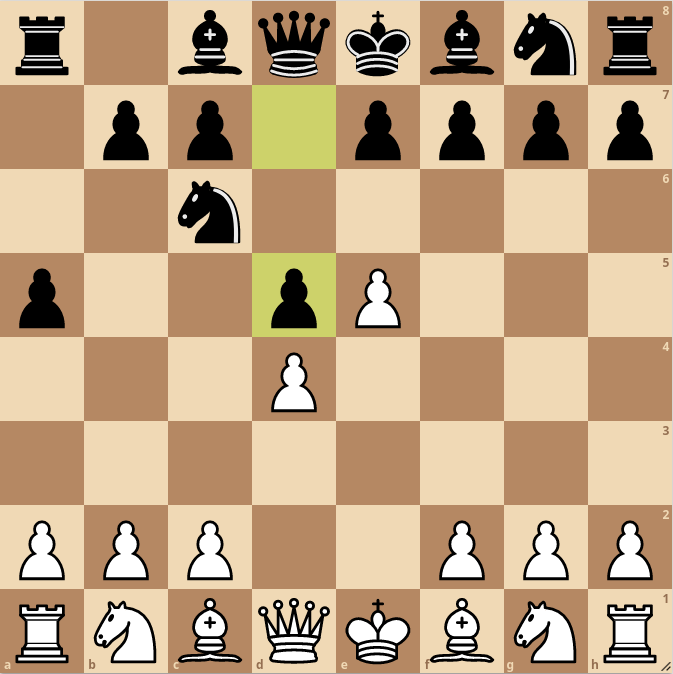
\includegraphics[width=0.35\textwidth]{img/input-boards2.png}
    \caption{Board example}
\end{figure}

\begin{figure}[H]
    \centering
    
\includegraphics[width=0.95\textwidth]{img/input-boards.png}
    \caption{The input state converted from the above example board}
\end{figure}

Notice how the last square shows the square were en passant is possible.
Grey padding was added to make a better visual presentation of the output planes.

The neural network will return the policy and the value of the position.
As described in the research part of this thesis, the value is a float between -1 and 1, and the 
policy is a 73x8x8 tensor of floats. This policy is then mapped to a dictionary, where keys are moves and 
the values are the probabilities of each move.

The neural network gets no information about the rules of chess, so it is necessary to filter
out the illegal moves. 

\begin{figure}[H]
    \centering
    
\includegraphics[width=0.95\textwidth]{img/output-planes/unfiltered.png}
    \caption{A subset of the 73 8x8 planes from the policy output. The brighter the pixel, the better the move.}
\end{figure}

\begin{figure}[H]
    \centering
    
\includegraphics[width=0.95\textwidth]{img/output-planes/filtered.png}
    \caption{The same subset, but with the illegal moves filtered out}
\end{figure}

The above two images were made using a trained model. The policy output of an untrained model with random weights 
looks like this:

\begin{figure}[H]
    \centering
    
\includegraphics[width=0.5\textwidth]{img/output-planes/random-model-unfiltered.png}
    \caption{Some output planes from an untrained model.}
\end{figure}

(Black padding was used instead of gray to make it clearer.)

This clearly shows the trained model has at least some level of understanding of which moves are legal, 
without giving it any knowledge about the rules of chess. The model isn't even told we're playing chess: it
learns the correct outputs completely on its own. 

\subsubsection{The evaluation step}

The value received from the neural network is now assigned to the leaf node.

\subsubsection{The backpropagation step}

The value from the leaf node is now also added to every selected node in the path from the root to the leaf node.
Concretely, for every selected edge in the path, the following values are changed:

\begin{itemize}
    \item The edge's input node's visit count is incremented by 1
    \item The edge's visit count is incremented by 1
    \item The edge's value is incremented by the value of the leaf node
\end{itemize}


\subsection{Creating the dataset}


\begin{figure}[H]
    \centering
    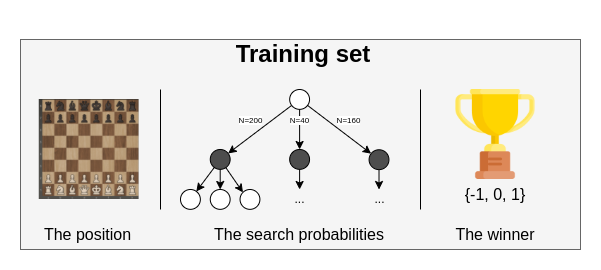
\includegraphics[width=0.7\textwidth]{img/trainingset.png}
    \caption{The training set consists of: the input state, the move probabilities, and the eventual winner}
\end{figure}

To improve the performance of the neural network, the algorithm needs to play against itself for a high amount of games.
Every move is saved to memory in a simple Python list. Once the game is over, the winner is added to every move in memory.
The whole game is then saved to a binary file in NumPy's .npy format. 
When a new game starts, the memory is cleared.

\subsubsection{Creating a dataset from puzzles}

Because creating the dataset is extremely time-consuming, I came up with the idea to also
create data from chess puzzles. The idea is to let the agent play from a certain given position (the puzzle), 
instead of from the start of the game, and see if the agent can find the correct solution.
This would in theory give the model a better understanding of common chess tactics, without having to play
whole games from start to finish.

A chess puzzle is a position with one simple goal: find the best move or sequence of moves.
Lichess.org, the open source chess website, has a huge database of over 2 million of these puzzles publicly available for free \cite{LichessOrgOpen}. 
These are the most common puzzle categories:

\begin{itemize}
    \item Mate-in-X: find the best moves to checkmate the opponent in a maximum of X moves
    \item Capturing one of the opponent's undefended pieces
    \item Getting a positional advantage
\end{itemize}

When creating the dataset, mate-in-1 and mate-in-2 puzzles were also added to the dataset. This is because these kinds of puzzles
end quickly (and are thus less time-consuming), and they have a clear winner: the player who can checkmate the opponent.
The Lichess database has over 400,000 puzzles of these two types. 

\subsection{Training the neural network}

\begin{figure}[H]
    \centering
    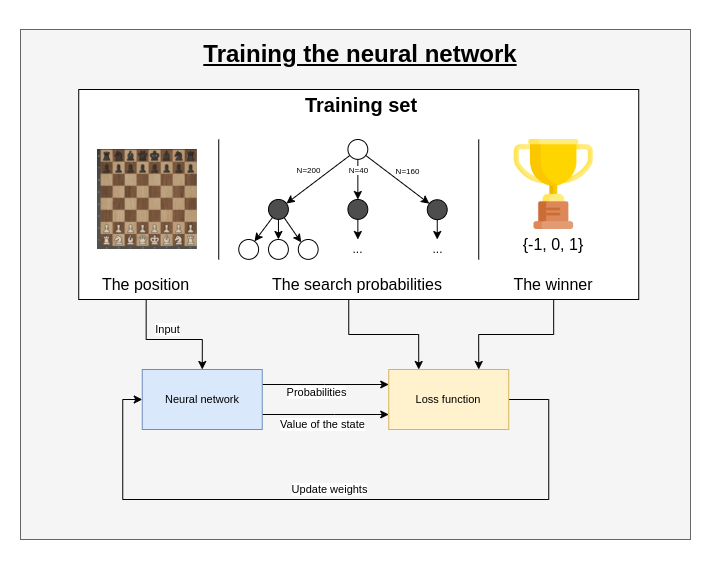
\includegraphics[width=0.9\textwidth]{img/training.png}
    \caption{The training pipeline}
\end{figure}

To train the neural network, every saved game's binary file is loaded 
into memory. The memory is shuffled to avoid the neural network accidentally learning
time dependent patterns. Random batches of the training set are then processed through the
neural network.

The position is used as the input to the neural network. The network's outputs are then 
compared to the move probabilities and the winner from the dataset:

\begin{itemize}
    \item The move probabilities are converted to a 73x8x8 tensor, which is compared with the output of the network
    \item The winner is compared with the value output of the network.
\end{itemize}

The training pipeline employs two separate loss functions. The policy head uses categorical cross-entropy
and the value head uses mean squared error.

\subsubsection{The first training session}

\begin{figure}[H]
    \centering
    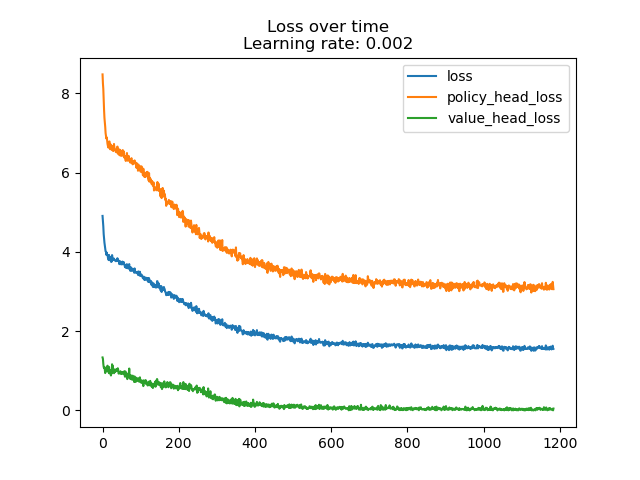
\includegraphics[width=0.6\textwidth]{img/first-training.png}
    \caption{First training session}
\end{figure}

Naturally, the first training session started with a random model. 
The dataset was created by running self-play for many hours, resulting in a dataset of around
76,000 positions. Training was performed with a learning rate of 0.002, and a batch size of 64.
The model uses the Adam optimizer.

After training, the model was saved to disk.

\subsubsection{The second training session}

The previous model was used as the starting point for the second training session.
A new dataset was made using only games created by that model. 
This time, due to time constraints, the dataset only had 50,000 positions.

\begin{figure}[H]
    \centering
    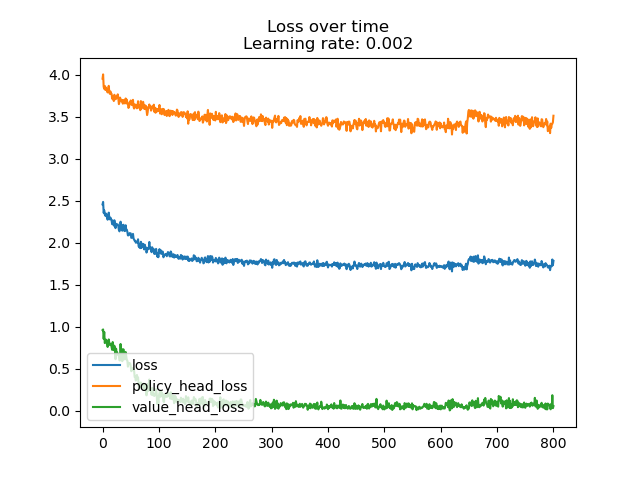
\includegraphics[width=0.6\textwidth]{img/second-training.png}
    \caption{Second training session}
\end{figure}

It's clear the model manages to learn something at the start of the training session,
but seems to plateau after 150 batches. Because the first training session started from 
a random model, it managed to learn a lot more before reaching a plateau after around 600 batches.

\subsection{Multiprocessing}

Because self-play is very time-consuming, there needed to be a way to play multiple games in parallel.

\subsubsection{Without multiprocessing}

\begin{figure}[H]
    \centering
    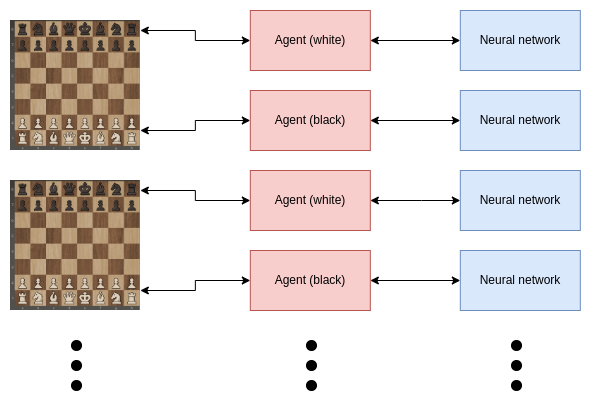
\includegraphics[width=0.65\textwidth]{img/without-multiprocessing.png}
    \caption{Self-play without multiprocessing}
\end{figure}

Previously, every game was played in its own process, but every agent needed to send predictions to a neural network.
This resulted in every process creating its own copy of the neural network. This is extremely heavy for the GPU, and
it's impossible to scale. Due to VRAM limits, only two games could be played in parallel on my system (RTX 3070).

\subsubsection{With multiprocessing}

\begin{figure}[H]
    \centering
    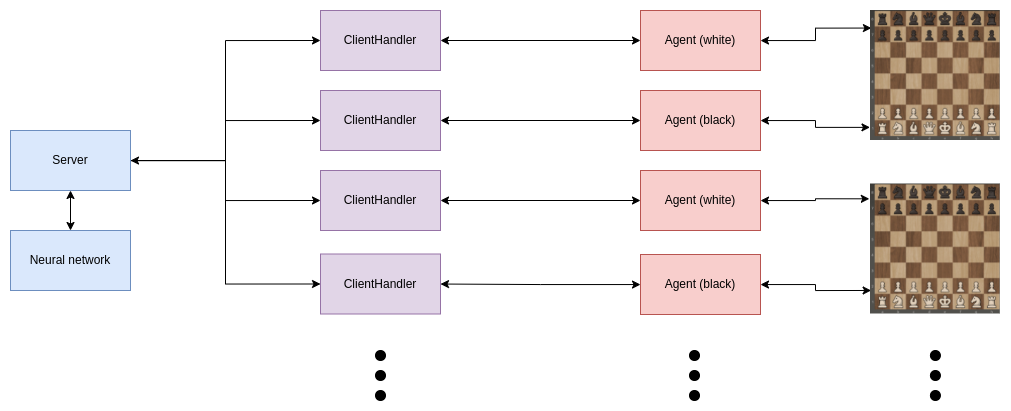
\includegraphics[width=0.95\textwidth]{img/with-multiprocessing.png}
    \caption{Self-play with multiprocessing}
\end{figure}

To solve the issue of parallel self-play, I created a client-server architecture with Python sockets.
The server side has access to the neural network. For every client (the self-play process), 
the server creates a ClientHandler in a new thread.

Here's how one client works:

\begin{enumerate}
    \item The MCTS algorithm runs 100s of simulations every move. Every simulation sends a chess position to the neural network.
    \item The agent sends the chess position through a socket.
    \item The ClientHandler receives the chess position and sends it to the server.
    \item The server calls the network's predict function and returns the outputs to the client handler.
    \item The ClientHandler sends the outputs back to the client.
\end{enumerate}

This socket communication does have a small overhead in both time and CPU usage, but it's much faster than the previous method
because it is much more scalable. Here's a comparison of the two methods, with the server running on the first system:

\begin{table}[H]
\resizebox{\textwidth}{!}{%
\begin{tabular}{lccll}
\cline{1-3}
\multicolumn{1}{|l|}{}                                  & \multicolumn{1}{c|}{\textbf{No multiprocessing}} & \multicolumn{1}{c|}{\textbf{With multiprocessing (8 games)}} &  &  \\ \cline{1-3}
\multicolumn{1}{|l|}{\textbf{RTX 3070 + Ryzen 7 5800H}} & \multicolumn{1}{c|}{50 simulations/sec}          & \multicolumn{1}{c|}{30 simulations/sec per game}             &  &  \\ \cline{1-3}
\multicolumn{1}{|l|}{\textbf{GTX 1050 + i7 7700HQ}}     & \multicolumn{1}{c|}{30 simulations/sec}          & \multicolumn{1}{c|}{15 simulations/sec per game}             &  &  \\ \cline{1-3}
                                                        & \multicolumn{1}{l}{}                             & \multicolumn{1}{l}{}                                         &  & 
\end{tabular}%
}
\caption{Comparison of multiprocessing and non-multiprocessing self-play}
\end{table}

With 8 games in parallel on the first system, I managed to get an average speed of $30 \cdot 8 = 240$ simulations per second.
The second system is much less powerful and needed to connect over Wi-Fi, but it still managed an average of $120$ simulations per second. 

\subsection{A GUI to play against the engine}

The GUI was based on a GitHub project that someone created for simply visualizing a chessboard with PyGame \cite{adefokunChessboardAhirajustice2022, pygame}.
I greatly improved and expanded that project to include a way for the player to interact with the board, play against an engine,
play against yourself, and more \cite{zjefferChessboardZjeffer2022}. I created a pull request to include my changes in the original author's GitHub project,
but it was declined due to being due extensive and out-of-scope for the project \cite{adefokunChessboard2022pull}.

Using this code, a GUI class was created for playing against the engine. The player can choose a color and play against
the engine. Clicking on a piece will highlight its square, clicking on another square will move the piece to that square.
Right-clicking will cancel the move.

\begin{figure}[H]
    \centering
    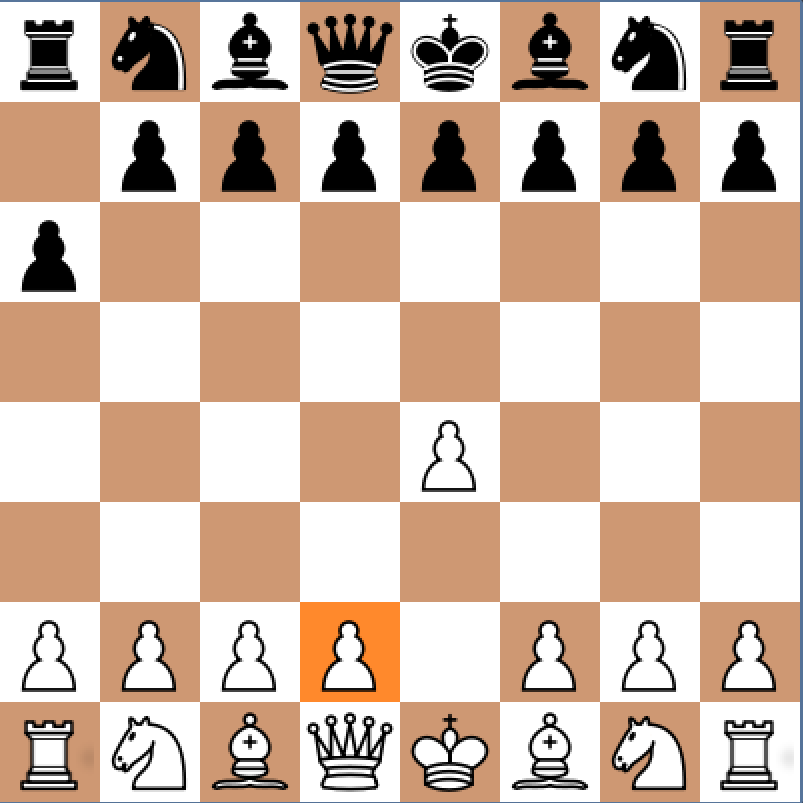
\includegraphics[width=0.5\textwidth]{img/chessboard-gui.png}
    \caption{Chessboard example when playing against the engine}
\end{figure}

Promoting a pawn can be done by simply moving a pawn to the last rank. A menu will pop up 
to choose the piece to promote to.

\begin{figure}[H]
    \centering
    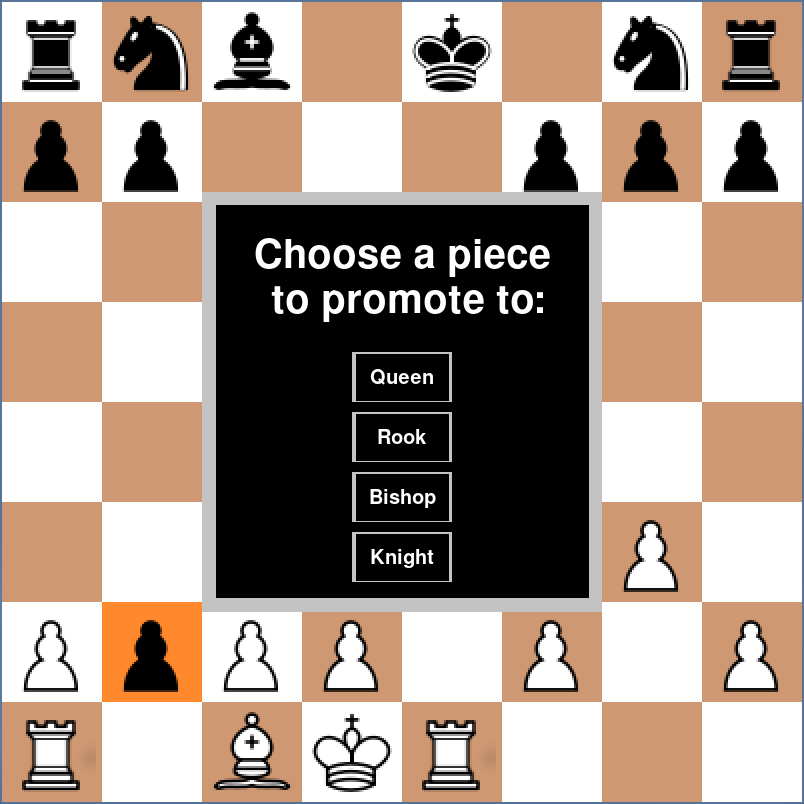
\includegraphics[width=0.5\textwidth]{img/chessboard-promotion.png}
    \caption{Promoting a pawn}
\end{figure}

\subsection{Docker images}

Because the amount of data needed to train the neural network is very large, two docker images were created:

\begin{itemize}
    \item A server image that runs the neural network and listens for clients.
    \item A client image that runs self-play and sends chess positions to the server.
\end{itemize}

With a docker-compose file, the server and client images can be easily started. The number of clients 
to run in parallel can be easily configured in that file.

It's recommended to run the server on a fast GPU-equipped system, and the clients on a system with many high-performance CPU cores.
The clients do not need a GPU to run self-play.

\subsection{The final project}

This section walks through all executable programs included in the project \cite{zjefferChessEngineDeep2022}.

\subsubsection{Creating your own untrained AI model}

\begin{minted}{text}
$ python rlmodelbuilder.py --help
usage: rlmodelbuilder.py [-h] [--model-folder MODEL_FOLDER] [--model-name MODEL_NAME]

Create the neural network for chess

options:
  -h, --help            show this help message and exit
  --model-folder MODEL_FOLDER
                        Folder to save the model
  --model-name MODEL_NAME
                        Name of the model (without extension)
\end{minted}

This will create a new model with the name <NAME> in the folder <FOLDER>.
The model parameters (amount of hidden layers, input and output shapes if you want to use the network for a different game, the amount of convolution filters, etc.)
can be changed by editing the config.py file.

\subsubsection{Creating a training set through self-play}

Creating the docker containers:

\begin{minted}{shell}
# in the repo's code/ folder:
docker-compose up --build
\end{minted}

This will create one server and the amount of clients that is configured in the docker-compose.yml file.
That file can also be used as a reference to deploy a Kubernetes cluster for parallel self-play with 
high scalability and reliability. 

Using the created GUI, it is possible to visualize the self-play of all these boards in real-time.
This can be done by settings the ``SELFPLAY\_SHOW\_BOARD'' environment variable in docker-compose.yml to ``true''.
For every replica of the client, a new PyGame window will open where the board will change in real-time. 

You can also manually run self-play or create data using puzzles:

\begin{minted}{text}
$ python selfplay.py --help
usage: selfplay.py [-h] [--type {selfplay,puzzles}] [--puzzle-file PUZZLE_FILE] 
    [--puzzle-type PUZZLE_TYPE] [--local-predictions]

Run self-play or puzzle solver

options:
    -h, --help            show this help message and exit
    --type {selfplay,puzzles}
                        selfplay or puzzles
    --puzzle-file PUZZLE_FILE
                        File to load puzzles from (csv)
    --puzzle-type PUZZLE_TYPE
                        Type of puzzles to solve. Make sure to set a 
                        puzzle move limit in config.py if necessary
    --local-predictions   Use local predictions instead of the server
\end{minted}

\subsubsection{Evaluating two models}

To determine whether your new model is better than the previous best, you can use the evaluate.py script.
It will simulate matches between the two models and record the wins, draws and losses.

In chess, white inherently has a slightly higher chance of winning because they can play the first move \cite{FirstmoveAdvantageChess2022}.
Therefore, to evaluate two models, each model will both play white and black an equal amount of times.

\begin{minted}{text}
$ python evaluate.py --help
usage: evaluate.py [-h] model_1 model_2 nr_games

Evaluate two models

positional arguments:
  model_1     Path to model 1
  model_2     Path to model 2
  nr_games    Number of games to play (x2: every model plays both white and black)

options:
  -h, --help  show this help message and exit
\end{minted}

\subsubsection{Playing against the AI}

\begin{minted}{text}
$ python main.py --help
usage: main.py [-h] [--player {white,black}] [--local-predictions] [--model MODEL]

options:
  -h, --help            show this help message and exit
  --player {white,black}
                        Whether to play as white or black. No argument means random.
  --local-predictions   Use local predictions instead of the server
  --model MODEL         For local predictions: specify the path to the model to use.
\end{minted}

This will start the GUI application to allow you to play against the engine. 

\subsection{Porting to C++}

Optimization is extremely important for chess engines, especially when the engine needs to play
against itself to create a dataset. That is why Python was not an ideal choice to implement this chess engine.

Currently, I'm writing a C++ version of the engine in my spare time \cite{zjefferChessdeeprlcpp2022}. Instead of TensorFlow Keras, I've opted to 
use PyTorch instead. So far, I've noticed that the C++ version with PyTorch manages to run the MCTS algorithm 
four times faster than the Python version: 200 simulations per second instead of 50.




%%%%% Reflection %%%%%
\newpage
\section{Reflection}

\subsection{Introduction}

This section is a reflection on the project. It will answer the following questions:

\begin{itemize}
    \item What are the strengths and weaknesses of this research project?
    \item Is the result of the project usable for corporations?
    \item What are the possible obstacles for companies that wish to implement this?
    \item What is the added value for companies?
    \item Which alternatives are there?
    \item Is there a socio-economic impact present?
    \item Is there opportunity for further research?
\end{itemize}

To help answer these questions, I have consulted with Dr. Thomas Moerland, a postdoctoral 
researcher at the Reinforcement Learning Group at Leiden University, in The Netherlands \cite{ThomasMoerlandPostdoc}. 
With his experience in researching AI and specifically Reinforcement Learning, he was able 
to give me some insights into how AlphaZero could impact society in industries besides gaming.

I have also asked questions to the following online communities:

\begin{itemize}
    \item The AI Stack Exchange community % TODO: link
    \item The Leela Chess Zero Discord community 
    \item The TalkChess forum, a forum affiliated with The Computer Chess Club (CCC)
\end{itemize}

\subsection{Strengths and weaknesses}

This project successfully implements the MCTS algorithm as modified by DeepMind for AlphaZero and their preceding work,
AlphaGo and AlphaGo Zero. The resulting chess engine can be played against using the GUI, and it can be used to create
a dataset for further improving the neural network. The project serves as an example of how AlphaZero's MCTS algorithm 
can be implemented in a chess engine using Python and consumer-grade hardware. 

The project offers a way to easily create your own neural network with the rlmodelbuilder.py script.
The code is written with modularity and adaptability in mind: by changing parameters in the config.py file, 
you can easily create a different model for chess, or for similar applications with different input and output shapes. 
The MCTS algorithm can be used as a reference if you want to implement it other applications.

The ultimate goal of this research project was to create a chess engine that is at least capable of winning
against amateur players of around 1000 ELO. This was not possible with my consumer-grade hardware: 
the chess engine still seems to play very randomly and has not found a good winning strategy. 
The biggest hurdle was the lack of computational resources to create a large dataset.

However, the project does offer a solution to create more data through self-play: with the docker containers, 
it is easy for other people to help create a dataset by deploying their own cluster of servers and clients. 
This way, a global dataset could be made by combining self-play data from volunteers around the world. 
It can then be used to train a new model. 

This is exactly how Leela Chess Zero operates: the developers created a simple program for volunteers to run,
which makes the latest model play against itself and uploads the data back to the developers. Once there is
enough data, the developers can retrain the model. By continuously repeating this process, Leela Chess Zero
slowly became a powerful chess engine on par with the best chess engines in the world \cite{TopChessEngine2022}.

\subsection{Is the result of the project usable in the corporate world?}

While AlphaZero and its variants have mostly been used in gaming applications, 
the project is not limited to this. For instance, AlphaGo has been used by Google
to properly ventilate their data centers more efficiently. The algorithm helped lower
data center cooling costs by 40\% \cite{decemberHasGoogleCracked2020}. 
It does this by periodically pulling data from many sensors and feeding that data to 
a deep neural network to predict how different combinations of potential actions
will affect future energy consumption \cite{HowAIHelps2018}.

Theoretically, this project can be used to solve virtually any problem that can be
defined as an agent acting upon an environment with discrete state and action spaces \cite{ReinforcementLearning2022a}.

Reinforcement learning in general has been used to solve a wide range of problems.
Many websites that have recommendation systems have already used reinforcement learning 
to improve which products get recommended to users \cite{nbroAnswerAreThere2020}. 
For example, Netflix uses contextual bandits to personalize artwork to the user \cite{blogArtworkPersonalizationNetflix2017,surmenokContextualBanditsReinforcement2017}.
This avoids the need for waiting to collect data from users, training a model,
waiting for an A/B test to conclude, to then finally recommend the best artwork.
By then, too many users have ignored an item they would have otherwise clicked on.

% TODO \cite{slaterAnswerAreThere2017}

% TODO: openai five

In the field of robotics, (deep) reinforcement learning can be used to teach a robot
through self-play to perform simple tasks that previously required manual programming.

\subsection{What are the possible obstacles for companies that wish to implement this?}

Depending on the application, the amount of data necessary to train a sufficiently powerful model
can be extremely large. It's necessary for the company to have a good infrastructure to 
create this data. Companies can also invest in cloud solutions like the Google Cloud Platform
to take advantage of their TPUs \cite{CloudComputingServices}.

Because these types of algorithms need to be trained through self-play, applications should be written
in a programming language that is capable of training and inferring neural networks, 
but should also be very performant and efficient. 
Fast, low-level programming languages like C++ often require much more development time
to create the same application compared to high-level programming languages like Python. 
This should also be factored into the development process.

AI frameworks like TensorFlow and PyTorch are available in both Python and C++, 
but documentation and support is lacking in the C++ versions. This means companies 
who wish to implement this type of application will need to hire C++ developers who
are also experienced with neural networks.

\subsection{What is the added value for companies?}

Options are always useful, and this project offers a way to solve problems 
using AI without having to manually collect data. The reinforcement learning agent 
will collect data for you by playing against itself. This means the algorithm will
get better in a ``fire-and-forget'' manner: just launch a cluster of self-play agents
and wait until it gathers enough data. You could create an automatic pipeline to
retrain the model after a set amount of time or after a certain amount of games.

\subsection{Which alternatives are there?}

For chess specifically, there are many chess engines that can be used for both analysis
and playing against. StockFish is the most popular, and as mentioned before, 
Leela Chess Zero is also open source and works the same way as AlphaZero. 

For industries other than the gaming industry, many problems are solvable by using
machine learning algorithms instead of reinforcement learning solutions. 
Supervised learning methods have a very wide range of applications, provided 
you have the data to train a model.

However, if you don't have a means to gather data, there are many reinforcement
learning algorithms other than AlphaZero:

\begin{itemize}
    \item Q-learning
    \item SARSA
    \item DQN
    \item Actor-Critic methods like A2C or A3C
    \item \dots
\end{itemize}

Currently, sending inputs from the client to the server for predicting outputs with 
the neural network happens through Python sockets. A good alternative for that is gRPC. 
It would allow the clients to directly call a method on the server without having to 
resort to Python sockets, which might be slower. \cite{IntroductionGRPC}

\subsection{Is there a socio-economic impact present?}

Sadly, algorithms like AlphaZero fail at solving even relatively simple problems like chess when the model 
does not have enough data to train on.  \cite{ThomasMoerlandPostdoc}. 
Given enough time and data, though, these types of algorithms can be used to achieve superhuman
performance in applications that were previously impossible to find optimal solutions for.

DeepMind's ultimate goal is to ``[...] solve intelligence, developing more general and capable 
problem-solving systems, known as artificial general intelligence (AGI).'' \cite{DeepMind}.
This is a slow and extremely difficult process, but DeepMind is confident AlphaZero and 
its variants are a big step towards that goal \cite{AlphaZeroSheddingNew}.

Others are more pessimistic about the progress DeepMind has made \cite{moerlandEmailExchangeTuur22, dukezhouAnswerAlphaZeroExample2018},
explaining that while AlphaGo (Zero) and AlphaZero have certainly been a huge breakthrough in their respective games, 
this does not mean their results a particularly big step towards AGI. 

\begin{quotation}
    I think there is a huge gap between the simple games we now solve and the 
    'artificial general intelligence' that DeepMind is trying to achieve.
    I believe that the most progress won't come from algorithms, but from calculations.
    For general AI, we need incredibly strong simulators where a huge amount of data
    can be passed through for a very long time. 
    Just like the millions of years of evolution our brains have been through, our brains
    have been gathering data non-stop throughout our lives. \cite{moerlandEmailExchangeTuur22}
\end{quotation}


\subsection{Is there opportunity for further research?}

While reinforcement learning has existed for a long time, deep reinforcement learning techniques 
have only recently been used. This is because of the lack of computational resources to train
a well-performing model. With high performance computing devices and cloud solutions getting cheaper
and more powerful, a lot of research opportunities open up.
Deep Reinforcement learning for autonomous driving has recently become an active area of research 
in both academia and industry \cite{DeepReinforcementLearning2022a}.

For this project specifically, there is still a lot of research opportunity to try to solve the problem
of creating a large enough dataset to train a sufficiently powerful model.

% TODO: expand this section




%%%%% Advice %%%%%
\newpage
\section{Advice}

\subsection{Introduction}

This section gives advice to people who wish to implement something similar to the project.
It includes recommendations and tips for when people want to program an application that uses
the algorithms and concepts researched in this thesis.

\subsection{When should you use this technology?}

This algorithm has a very specific purpose. It should only be used in situations where
both the action space and state space are discretely defined. Both of these should also
be relatively small, as bigger action spaces and state spaces will require much more 
data to successfully train a model. 
Therefore, it is important to keep the problem as simple as possible. 

\subsection{Recommendations}

When you want to implement AlphaZero or similar algorithms, it is recommended to
prioritize writing code in the most efficient way possible. Every step of the algorithm
should be programmed with multiprocessing and multithreading in mind. Furthermore,
the choice of programming language should be considered carefully. While most AI 
frameworks are primarily written for use in Python, and most documentation is written
for Python, the language just isn't fast enough for something that needs this much data through self-play. 
C++ would be a better choice.

As was apparent from the results of the research project, generating training data 
takes a very long time. A good solution to this problem is to first pretrain the model
on a small dataset. This will result in a model that is at least slightly familiar 
with the environment. Without a pretrained model, the algorithm will start from nothing
and make completely random actions. With a pretrained model, the algorithm will have some 
idea on what decisions to make based on the data it was given in pretraining.

% TODO

\subsection{Tips when programming a similar application}

This section will give some useful tips for programming an application that uses
AlphaZero's MCTS algorithm. 

\subsubsection{Creating the tree data structure}

The MCTS algorithm requires a tree to be constructed. As mentioned before, the nodes of the tree
are the positions of the game, and the edges between those nodes are the actions that can be taken
from those positions. 

It is important to avoid memory management issues when creating the tree. The MCTS algorithm 
can create quite large trees, especially when using hundreds of simulations. Every node object
should therefore only include the necessary data. For example, a very early version of my MCTS algorithm 
included all previous moves of the game in every node, creating a huge memory leak. This was fixed
by only storing the current board state as a FEN string in each node.

\subsubsection{Programming the MCTS algorithm}

When programming the MCTS algorithm, it is crucial to make every step as efficient as possible.
In the expansion step of the algorithm, the state of the leaf node should be converted to an object
that can be used as an input in the neural network. The function that converts the leaf's state 
can be very slow if it's not programmed efficiently. As that function needs to be called for every
simulation, every line of code should be optimized for speed.

Calling the neural network is definitely the slowest step of the algorithm. A good way to take 
advantage of this is to send batches of data to the network instead of one input at a time. 
This can be done by creating multiple threads to ``crawl'' through the tree at the same time 
during the selection step of the algorithm. 
Once every thread has finished by finding a leaf node, every leaf node can be sent to the network at once. 
For every output received by the neural network, a thread can again be started for the third and fourth steps. 
This will result in a significant speedup. 
The difficulty of programming this is mainly making sure the ``crawlers'' during the selection step
don't all select the same nodes. That would result in a less explored MCTS tree.

\subsubsection{Choosing the right input for the neural network}

As mentioned in the technical research part of this thesis, I opted for a smaller input
shape than the one defined in AlphaZero's paper. This is because I wanted to make the 
neural network as fast as possible. 

You should carefully consider what data the neural network would need to make a decision, 
based on the problem you're trying to solve. For example: when Google used AlphaGo to make
their data center's temperature control more efficient, they opted to use the sensors in the
data center as inputs to the neural network. 
You should make sure to omit any unnecessary data from the input.

%%%%% Conclusion %%%%%
\newpage
\section{Conclusion}

This thesis was created to critically evaluate my research project that tried to 
answer the question ``How to create a chess engine using deep reinforcement learning''.
The aim of the project was to create a chess engine based on DeepMind's AlphaZero in
Python with TensorFlow Keras. This was attempted by programming the MCTS algorithm 
and a neural network that can train on data collected from self-play. 
The ultimate goal of the project was not to create a chess engine that was capable of 
beating AlphaZero, but rather to create a simple version of AlphaZero that could 
beat amateur chess players of around 1000 ELO. 

Sadly, the resulting chess engine has not managed to reach this goal.
This is because of the lack of computational resources necessary to create a big enough
dataset through self-play. However, this thesis does offer some solutions to this problem:

\begin{itemize}
    \item Pretrain the model on a small dataset
    \item Use docker containers to set up a cluster of self-play agents
\end{itemize}

This thesis also serves as a warning to people who wish to implement similar algorithms
without having the necessary access to powerful hardware. It recommends investigating certain 
alternatives to AlphaZero, such as other reinforcement techniques like Q-learning, SARSA, and DQN,
but also supervised learning techniques if training data is available.




%%%%% Bibliography %%%%%
\newpage
\section{Bibliography}
\renewcommand{\bibname}{}
\printbibliography[heading=none]

%%%%% Appendix %%%%%
\newpage
\section{Appendix}

\subsection{Report guest speaker: ML6}

\subsubsection{Introduction}

On the 20th of January, I attended a very interesting talk by Matthias Feys, 
CTO of ML6. ML6 is an AI consultancy company based in Belgium, Germany, The Netherlands 
and Switzerland that serves customers across Europe. They have more than 90 
machine learning \& data engineering experts and are the largest and fastest 
growing AI company in Europe. 

The talk was about how the company tries to increase the explainability of their AI 
solutions. 

\subsubsection{What is Explainable AI?}

The inner workings of how an AI gets to a decision is often very difficult to explain.
Say you have some inputs and a neural network that takes those inputs and produces
one output: Yes or No. Without explainability, you can't tell the customer why the 
network makes the decision. The customer just has to take your word for it.

An improvement to the above example is instead of outputting a boolean value, 
a percentage could be used instead. This would allow the customer to understand
how sure the network is of its decision.

While AI technology is improving extremely quickly, adoption of these technologies
by other companies is often still a hurdle to overcome. Here are three scenarios in 
which Explainable AI can drive adoption. All of these scenarios have the goal of
building trust in the AI.

\begin{enumerate}
    \item AI is weaker than human
    \item AI is on par with human
    \item AI is stronger than human
\end{enumerate}

\subsubsection{AI is weaker than human}

In this scenario, adoption is very difficult, which is why explainability
will be primarily about improving the AI. By explaining how the AI makes a decision,
the customer can understand how they can help improve it. 

You can visualize the outputs of a model. For example: drawing lines and bounding 
boxes around the output of a neural network is a great way to show what the 
contribution of the model is.

You can improve the model by capturing lots of data, and either letting the customer label
the data themselves, or by fixing incorrect labels. This is called Active Learning, and it
focuses on the data where the model is weak. 
While waiting for a model to improve, you can manually create a simpler model that can
solve the specific edge case that went wrong before.

\subsubsection{AI is on par with human}

When the AI is as good as the human counterpart, you want to build trust in the
AI by discussing how it works. It's difficult to convince someone to consider 
using the AI over the human solution if they are equally valid options. 

In this scenario, explainability can help humans to use the result of the AI 
to their advantage. You're basically letting the AI and the human work together
to solve a problem.


\subsubsection{AI is stronger than human}

Stronger than human performance is great, but it's better if you can also explain
why it's the better option. Explainability here is about explaining a complicated
concept and informing humans.

The information you can learn from an AI is incredibly useful to companies in order
to improve their machines, processes, and products. 

\subsubsection{Five generic design patterns}

Here are 5 tips that are useful for explaining AI.

\begin{enumerate}
    \item Problem reframing
    \item Interpretable models
    \item Feature attribution
    \item Transparency \& transferability
    \item Intuitive visualizations
\end{enumerate}

\textbf{Problem reframing}

It's often better to completely reframe the problem before you start to think about
programming an AI to solve it. For example: when a customer asks to classify whether
a car is damaged or not, you can reframe the problem as an object detection problem.
An object detector can then be trained to detect specific locations of damage on the car.
This still answers the customer's initial needs, but is much easier to explain.

\textbf{Interpretable models}

Some models are generally more interpretable than others. Linear models, for example,
can be very easy to interpret, but these aren't very performant. LSTMs on the other hand,
can be very performant, but they are hard to interpret. It's crucial to find a correct
balance between both performance and interpretability. AI architectures can be combined
to solve a problem in a way that is both performant and easy to understand.

\textbf{Feature attribution}

It's important to understand which features are contributing the most or the least 
to the output of the model. For example: if you have a model that recommends a product,
you can show which features were had the most impact when recommending that specific product.
This can be done with techniques like SHAP values, saliency maps or LIME.

\textbf{Transparency \& transferability}

If the data changes drastically, for example due to a crisis like the coronavirus, the model might not be relevant anymore.
If a model uses another model, it is important that the first model is explainable as well. 
Validation of data is also very important: if the data is filled with mistakes, 
the output can not be trusted. That is why it's necessary to run a standard set of checks
on the data to uphold the quality of the dataset.

\textbf{Intuitive visualizations}

For example, when a model recommends a product, a visual representation can be shown of 
other products that are similar to the recommended product, from most similar to least similar.
This gives the customer a good sense of how it ranks products to your preferences.

For computer vision, saliency maps can show the importance of each pixel in the image when 
making a decision.

\subsubsection{Conclusion}

The main conclusion of the talk was that explainable AI is not just about using SHAP to explain
the features, but it is about much more than that.
Explainability is not just part of developing a model, 
it is present in the whole pipeline from start to finish: it starts with the framing of the problem
and ends with the user interface and user experience.

The goal is to increase trust and adoption.

\subsubsection{Critical reflection}

I thought it was a very interesting talk about a problem that isn't always given adequate 
attention in the AI community. It is also something I am personally guilty of: when developing
an AI, explainability is one of the last things I think of, when it should be part of the 
developing process from the start. For example, my bachelor thesis about creating a chess engine using deep reinforcement learning
is a project where almost no explainability is possible. This makes developing the AI 
very difficult, as it's not clear why the model makes its decisions. 

I was particularly intrigued by the way saliency maps can be used to explain the importance
of groups of pixels in an image [1]. This way, mistakes that a model makes can be easily visualized:
if a group of pixels is deemed as important by the model, but it's a false positive, actions can 
be taken to improve the model based on that edge case.


\subsubsection{Sources}

[1] ``Saliency map'' Wikipedia, Oct. 2021. [Online]. Available: https://en.wikipedia.org/w/index.
php?title=Saliency\_map\&oldid=1049691575 (visited on 04/16/2022)


\end{document}